\textbf{Problem 1. Flow in a Channel}

Let us consider a channel with the following cross-section:
\begin{figure*}[h!]
\centering
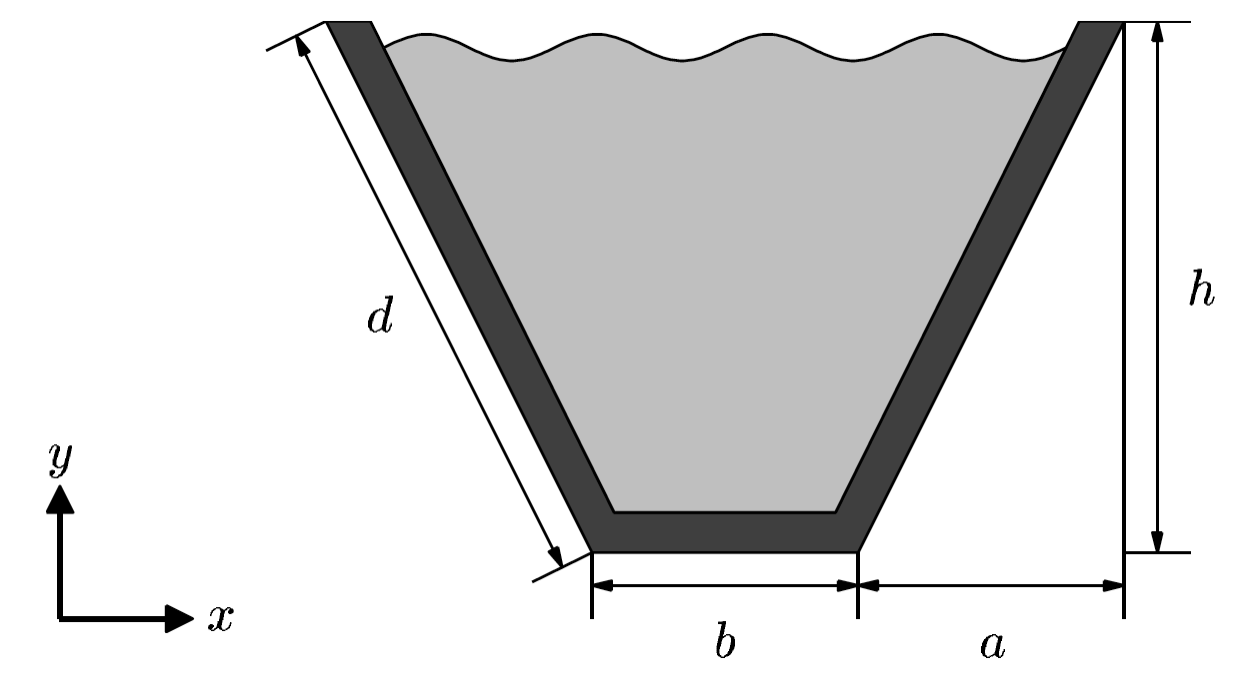
\includegraphics[width=0.5\textwidth]{figures/prj1_qn1_channel.png}\\
\caption{}
\label{prj1_qn1_channel}
\end{figure*}

where $b$ and $h$ are defined, and $l = b + 2d$ is assumed to be a constant.  Given $b$ and $h$, the other geometrical parameters can be calculated:
\begin{align}
    a &= \sqrt{\frac{1}{4}(l-b)^2-h^2} \\
    d &= \frac{1}{2}(l-b)
\end{align}

A fully developed flow can be reduced to Poisson's equation for the velocity component $u$ normal to the channel cross-section:
\begin{align}
    -\nabla^2u = \frac{g\sin\alpha}{\nu}
    \label{poisson}
\end{align}

where $\alpha$ is the tilt of the channel, $g$ is the gravitational constant and $\nu$ is the kinematic viscosity.  For simplicity's sake, we assume in this problem that $-\nabla^2u = 1$.  The velocity is zero (no-slip condition) along the walls of the channel and on the free surface a zero-stress condition $(\partial_\eta u = 0)$ is applied.

Due to symmetry, only half the channel section need be considered (Fig. \ref{prj1_qn1_coordtransform}).  We map the half-domain $\Omega$ of this half-channel section to a square domain $\hat{\Omega}$ and solve the equations using a finite difference method on $\hat{\Omega}$.  The boundary conditions are as follows:
\begin{align}
    \begin{cases}
        \partial_\eta u = 0, & \text{in $AB$ and $AD$} \\
        u = 0, & \text{in $BC$ and $CD$}
    \end{cases}
\end{align}

\begin{figure*}[h!]
\centering
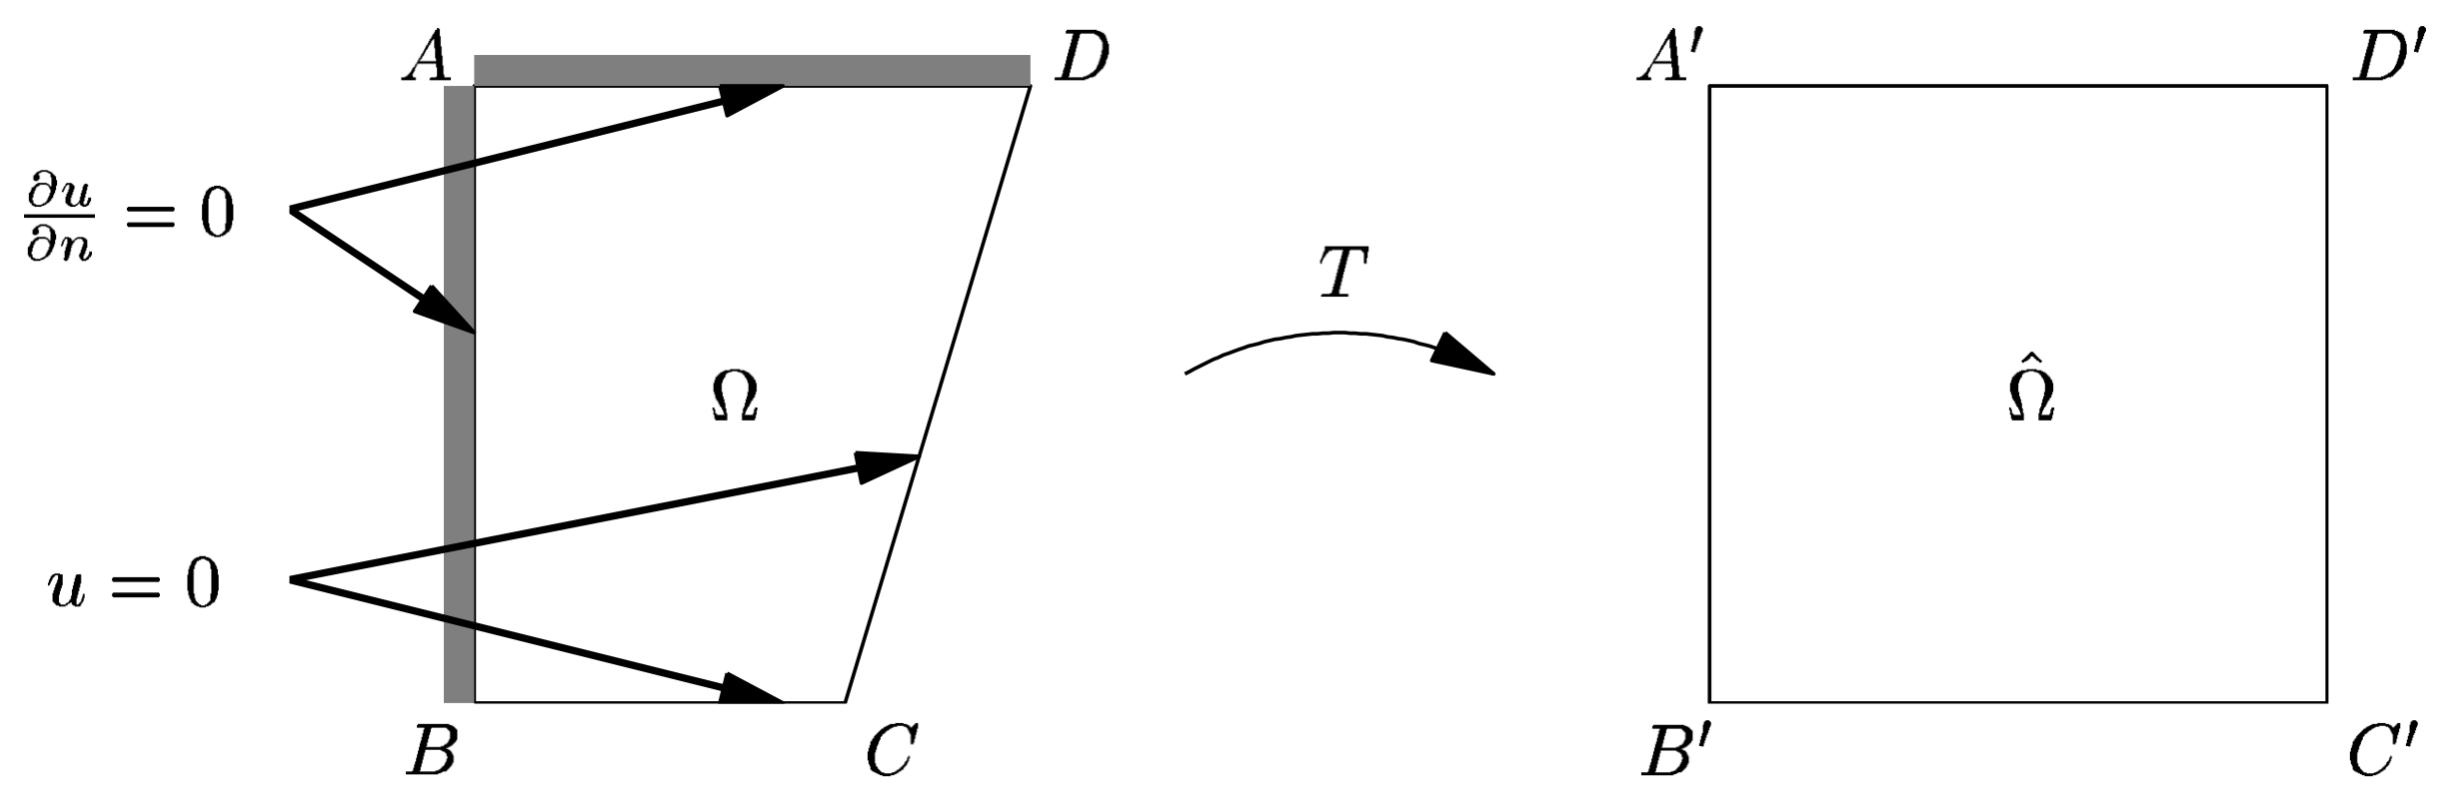
\includegraphics[width=0.7\textwidth]{figures/prj1_qn1_coordtransform.png}\\
\caption{}
\label{prj1_qn1_coordtransform}
\end{figure*}

We use a regular grid with $N\times N$ points in the computational domain, given square cells of size $\Delta\xi = \Delta\eta = \frac{1}{N-1}$.  This therefore implies that the transformed domain is square in nature as well, with bounds at (0,0), (0,1), (1,0) and (1,1).  We take point $B$ and $B'$ to be $(0,0)$ in both domains respectively for our coordinate transformation purposes.

\begin{enumerate}[label=(\roman*),leftmargin=*,itemsep=0mm]
    
    \item Let us perform the coordinate transformation such that $(x,y)$ coordinates in the $\Omega$ domain can be mapped to $(\xi,\eta)$ coordinates on the $\hat{\Omega}$ domain.  Given that the coordinates of $\eta$ remain unchanged with $y$, it is trivial to conclude that
    \begin{align}
        \eta = \frac{y}{h}
    \end{align}
    
    However, we see that the transformation of $x\rightarrow\xi$ is dependent on y
    \begin{align*}
        \xi = f(y) \cdot x
    \end{align*}
    
    such that when $\xi=1$, we have that
    \begin{align*}
        f(y) \cdot \left(\frac{b}{2} + a\cdot\frac{y}{h} \right) &= 1 \\
        \therefore f(y) &= \frac{1}{b/2 + ay/h} = \frac{2h}{bh + 2ay} \\
        &= \frac{h}{\frac{bh}{2} + y\sqrt{\frac{1}{4}(l-b)^2-h^2}}
    \end{align*}
    
    Therefore, we have that
    \begin{align}
        \xi = \frac{xh}{\frac{bh}{2} + y\sqrt{\frac{1}{4}(l-b)^2-h^2}}
    \end{align}
    
    Now, performing this coordinate transformation, we must also transform the Poisson equation and the boundary conditions as well. This requires us to express $(x,y)$ in terms of $(\xi,\eta)$.  Therefore, reversing the equations gives us
    \begin{align}
        y &= h\eta \\
        x &= \frac{\xi}{h}\left( \frac{bh}{2} + y\sqrt{\frac{1}{4}(l-b)^2-h^2} \right) \nonumber \\
        &= \xi \left(\frac{b}{2} + \eta\sqrt{\frac{1}{4}(l-b)^2-h^2} \right)
    \end{align}
    
    Therefore, we see that
    \begin{align}
        y_\eta &= h \label{yeta}\\
        x_\xi  &= \frac{b}{2} + \eta\sqrt{\frac{1}{4}(l-b)^2-h^2} = \frac{b}{2} + \eta a\\
        x_\eta &= \xi\sqrt{\frac{1}{4}(l-b)^2-h^2} = \xi a \\
        x_{\xi\eta} &= \sqrt{\frac{1}{4}(l-b)^2-h^2} = a \label{xxieta}
    \end{align}
    
    And all other 1st- and 2nd-order derivatives are equal to zero.  Thus, we see from the notes that we transform the equation (\ref{poisson}) to:
    \begin{align}
        c_1u_{\xi\xi} -2c_2u_{\xi\eta} + c_3u_{\eta\eta} + c_4u_\eta + c_5u_\xi = -J^2
    \end{align}
    
    where $c_1$, $c_2$, $c_3$, $c_4$ and $c_5$ are given by, from equations (\ref{yeta}-\ref{xxieta})
    \begin{align}
        c_1 &= x_\eta^2 + y_\eta^2 = \xi^2 a^2 + h^2 \\
        c_2 &= x_\xi x_\eta + y_\xi y_\eta = x_\xi x_\eta
        = \frac{b\xi}{2} a + \xi\eta a^2 \\
        c_3 &= x_\xi^2 + y_\xi^2 = x_\xi^2 = \frac{b^2}{4} + b\eta a + \eta^2a^2 \\
        c_4 &= 0 \\
        c_5 &= \frac{2c_2ha}{J} = 2a^2\xi \\
        J &= x_\xi y_\eta - x_\eta y_\xi = x_\xi y_\eta = \frac{bh}{2} + \eta ha
    \end{align}
    
    Along the $A'$-$B'$ boundary where $\xi$ is constant, we see that $\mathbf{n} = (n^x,n^y)$ is given y
    \begin{align*}
        \mathbf{n} = \frac{1}{\sqrt{x_\eta^2 + y_\eta^2}}(y_\eta,-x_\eta) = \frac{1}{\sqrt{\xi^2a^2 + h^2}} (h,-\xi a)
    \end{align*}
    
    Therefore, we transform $\partial_\eta u = 0$ into
    \begin{align*}
        (y_\eta n^x - x_\eta n^y)u_\xi + x_\xi n^y u_\eta &= 0 \nonumber \\
        \therefore (hy_\eta + \xi a x_\eta)u_\xi - \xi a x_\xi u_\eta &= 0 \\
        \xi a \left(\frac{b}{2} + \eta a\right) u_\eta
        &= (h^2 + \xi^2 a^2) u_\xi
    \end{align*}
    
    Recognizing that at the $A'$-$B'$ boundary, $\xi=0$, this equation simplifies down to
    \begin{align}
        u_\xi = 0
    \end{align}
    
    Along the $A'$-$D'$ boundary where $\eta$ is constant, we see that $\mathbf{n} = (n^x,n^y)$ is given y
    \begin{align*}
        \mathbf{n} = \frac{1}{\sqrt{x_\xi^2 + y_\xi^2}}(-y_\xi,x_\xi) = (0,1)
    \end{align*}
    
    Therefore, we transform $\partial_\eta u = 0$ into
    \begin{align*}
        x_\xi n^y u_\eta - x_\eta n^y u_\xi &= 0 \\
        \therefore \left(\frac{b}{2} + \eta a\right) u_n &= \xi a u_\xi
    \end{align*}
    
    Recognizing that at the $A'$-$D'$ boundary, $\eta=1$, this equation simplifies down to
    \begin{align}
        \left(\frac{b}{2} + a\right) u_\eta &= \xi a u_\xi
    \end{align}
    
    And along the $B'$-$C'$ and $C'$-$D'$ boundaries, we have that $u = 0$.
    
    \item Now, we find the 2nd-order accurate finite difference scheme for the discretization of all the derivative terms in the interior of the domain (i.e. $2 \leq i,j \leq N-1$).
    \begin{align}
        c_1u_{\xi\xi} |_{i,j} 
        &= (N-1)^2 c_1|_{i} \cdot \left(u_{i+1,j} + u_{i-1,j} - 2 u_{i,j} \right)
    \end{align}
    \begin{align}
        c_2u_{\xi\eta} |_{i,j} &= \frac{(N-1)^2}{4} c_2 |_{i,j} \cdot (u_{i+1,j+1} + u_{i-1,j-1} - u_{i+1,j-1} - u_{i-1,j+1})
    \end{align}
    \begin{align}
        c_3u_{\eta\eta} |_{i,j} &= (N-1)^2 c_3|_{j} \cdot (u_{i,j+1} + u_{i,j-1} - 2u_{i,j})
    \end{align}
    \begin{align}
       c_5u_\xi |_{i,j} &= \frac{N-1}{2} c_5|_j (u_{i+1,j}-u_{i-1,j})
    \end{align}
    
    When $i=1, 1 < j < N$, we use the 2nd-order downwind in the $\xi$-direction for equation (20)
    \begin{align}
        u_\xi
        = (N-1) \left( \frac{3}{2}u_{1,j} - 2u_{2,j} + \frac{1}{2}u_{3,j} \right) = 0
    \end{align}
    
    When $i < N-1, j = N$, we use the 2nd-order downwind in the $\xi$-direction and 2nd-order upwind in the $\eta$-direction for equation (21).  We note that for $i=1$, $\xi = 0$ and therefore there the only variable of concern is $\eta$.  Thus, we obtain
    \begin{align}
        \left(\frac{b}{2} + a\right) \left(3u_{i,N-2} - 4u_{i,N-1} + u_{i,N} \right)
        - \frac{i-1}{N-1} a \left(-3u_{i,N} + 4u_{i+1,N} - u_{i+2,N} \right) = 0
    \end{align}
    
    When $i = N-1, j = N$, we use the 2nd-order central difference in the $\xi$-direction and 2nd-order upwind in the $\eta$-direction for equation (21).
    \begin{align*}
        \left(\frac{b}{2} + a\right) \left(3u_{N-1,N-2} - 4u_{N-1,N-1} + u_{N-1,N} \right)
        - \frac{i-1}{N-1} a \left( u_{N,N} - u_{N-2,N} \right) = 0
    \end{align*}
    
    And since $u_{N,N} = 0$, we have that
    \begin{align}
        \left(\frac{b}{2} + a\right) \left(3u_{N-1,N-2} - 4u_{N-1,N-1} + u_{N-1,N} \right)
        + \frac{i-1}{N-1} a u_{N-2,N} = 0
    \end{align}
    
    And when $i=N$ or $j=1$, we have that $u=0$.
    
    Next, we solve for the approximate flow rate $\hat{Q}$ in the $(\xi,\eta)$ coordinates using the 2D trapezoidal method:
    \begin{align*}
        \hat{Q} &= \iint_\Phi u \dd{x}\dd{y} 
        = \int_0^1\int_0^1 u \dd{\xi} \left(\frac{b}{2} + \eta a\right) \cdot h\dd{\eta} \\
        &= \frac{h}{4(N-1)^2}\sum_{j=1}^{N-1} \sum_{i=1}^{N-1} 
        \left[ (u_{i,j}+u_{i+1,j})\left(\frac{b}{2} + \eta_{j} a\right)
        + (u_{i,j+1}+u_{i+1,j+1})\left(\frac{b}{2} + \eta_{j+1} a\right)\right]
    \end{align*}
    
    \item If we sum up the total number of nodes, we see that there are a total of $N^2$ equations, for $N^2$ nodes and therefore the system of linear-equations is critical.  Let us now break down the weights in the matrix for a node $N_{i,j}$.
    
    For the interior nodes, the non-zero entries at the row $N_{i,j}$ are
    \begin{itemize}[noitemsep,nolistsep]
        \item Column $i + (j-1)N$ has value $a_{i + (j-1)N} = -2(c_1+c_3)(N-1)^2$
        \item Column $(i-1) + (j-1)N$ has value $a_{i-1 + (j-1)N} = c_1(N-1)^2-c_5\frac{N-1}{2}$
        \item Column $(i+1) + (j-1)N$ has value $a_{i+1 + (j-1)N} = c_1(N-1)^2+c_5\frac{N-1}{2}$
        \item Column $i + (j-2)N$ has value $a_{i + (j-2)N} = c_3(N-1)^2$
        \item Column $i + jN$ has value $a_{i + jN} = c_3(N-1)^2$
        \item Column $i-1 + (j-2)N$ has value $a_{i-1 + (j-2)N} = -0.5c_2(N-1)^2$
        \item Column $i+1 + jN$ has value $a_{i+1 + jN} = -0.5c_2(N-1)^2$
        \item Column $i+1 + (j-2)N$ has value $a_{i+1 + (j-2)N} = 0.5c_2(N-1)^2$
        \item Column $i-1 + jN$ has value $a_{i-1 + jN} = 0.5c_2(N-1)^2$
    \end{itemize}
    
    And on the right hand side we solve for $J_{i + (j-1)N}$
    
    For the boundary nodes where $i=1, 1 < j < N$, the non-zero entries at the row $N_{1,j}$ are
    \begin{itemize}[noitemsep,nolistsep]
        \item Column $1 + (j-1)N$ has value $a_{1 + (j-1)N} = 3$
        \item Column $2 + (j-1)N$ has value $a_{2 + (j-1)N} = -4$
        \item Column $3 + (j-1)N$ has value $a_{3 + (j-1)N} = 1$
    \end{itemize}
    
    And on the right hand side we solve for 0.
    
    For the boundary nodes where $i < N-1, j = N$, the non-zero entries at the row $N_{1,j}$ are
    \begin{itemize}[noitemsep,nolistsep]
        \item Column $i + (N-3)N$ has value $a_{i + (N-3)N} = a+b/2$
        \item Column $i + (N-2)N$ has value $a_{i + (N-2)N} = -4(a+b/2)$
        \item Column $i + (N-1)N$ has value $a_{i + (N-1)N} = 3a(i-1)/(N-1) + 3(a+b/2)$
        \item Column $i+1 + (N-1)N$ has value $a_{i+1 + (N-1)N} = -4a(i-1)/(N-1)$
        \item Column $i+2 + (N-1)N$ has value $a_{i+2 + (N-1)N} = a(i-1)/(N-1)$
    \end{itemize}
    
    And on the right hand side we solve for 0.
    
    For the boundary nodes where $i < N-1, j = N$, the non-zero entries at the row $N_{1,j}$ are
    \begin{itemize}[noitemsep,nolistsep]
        \item Column $i + (N-3)N$ has value $a_{i + (N-3)N} = 3(a+b/2)$
        \item Column $i + (N-2)N$ has value $a_{i + (N-2)N} = -4(a+b/2)$
        \item Column $i + (N-1)N$ has value $a_{i + (N-1)N} = a+b/2$
        \item Column $i-1 + (N-1)N$ has value $a_{i-1 + (N-1)N} = a(i-1)/(N-1)$
    \end{itemize}
    
    And on the right hand side we solve for 0.
    
    And for all other nodes, we have that column $i + (j-1)N$ has value 1 and on the right hand side we solve for 0.
    
    \item We write a program that solves this problem in Julia code, see Fig. \ref{prj1_qn1f_b0d5}a for the solution when $l=3.0$, $b=0.5$, $h=1.0$ and $N=21$.  For this case, $\hat{Q} = 0.12481$, although it is also apparent that as $N$ increases, the solution converges towards $\hat{Q} = 0.11496$ which is the actual solution.

    \begin{figure*}[h!]
    \centering
    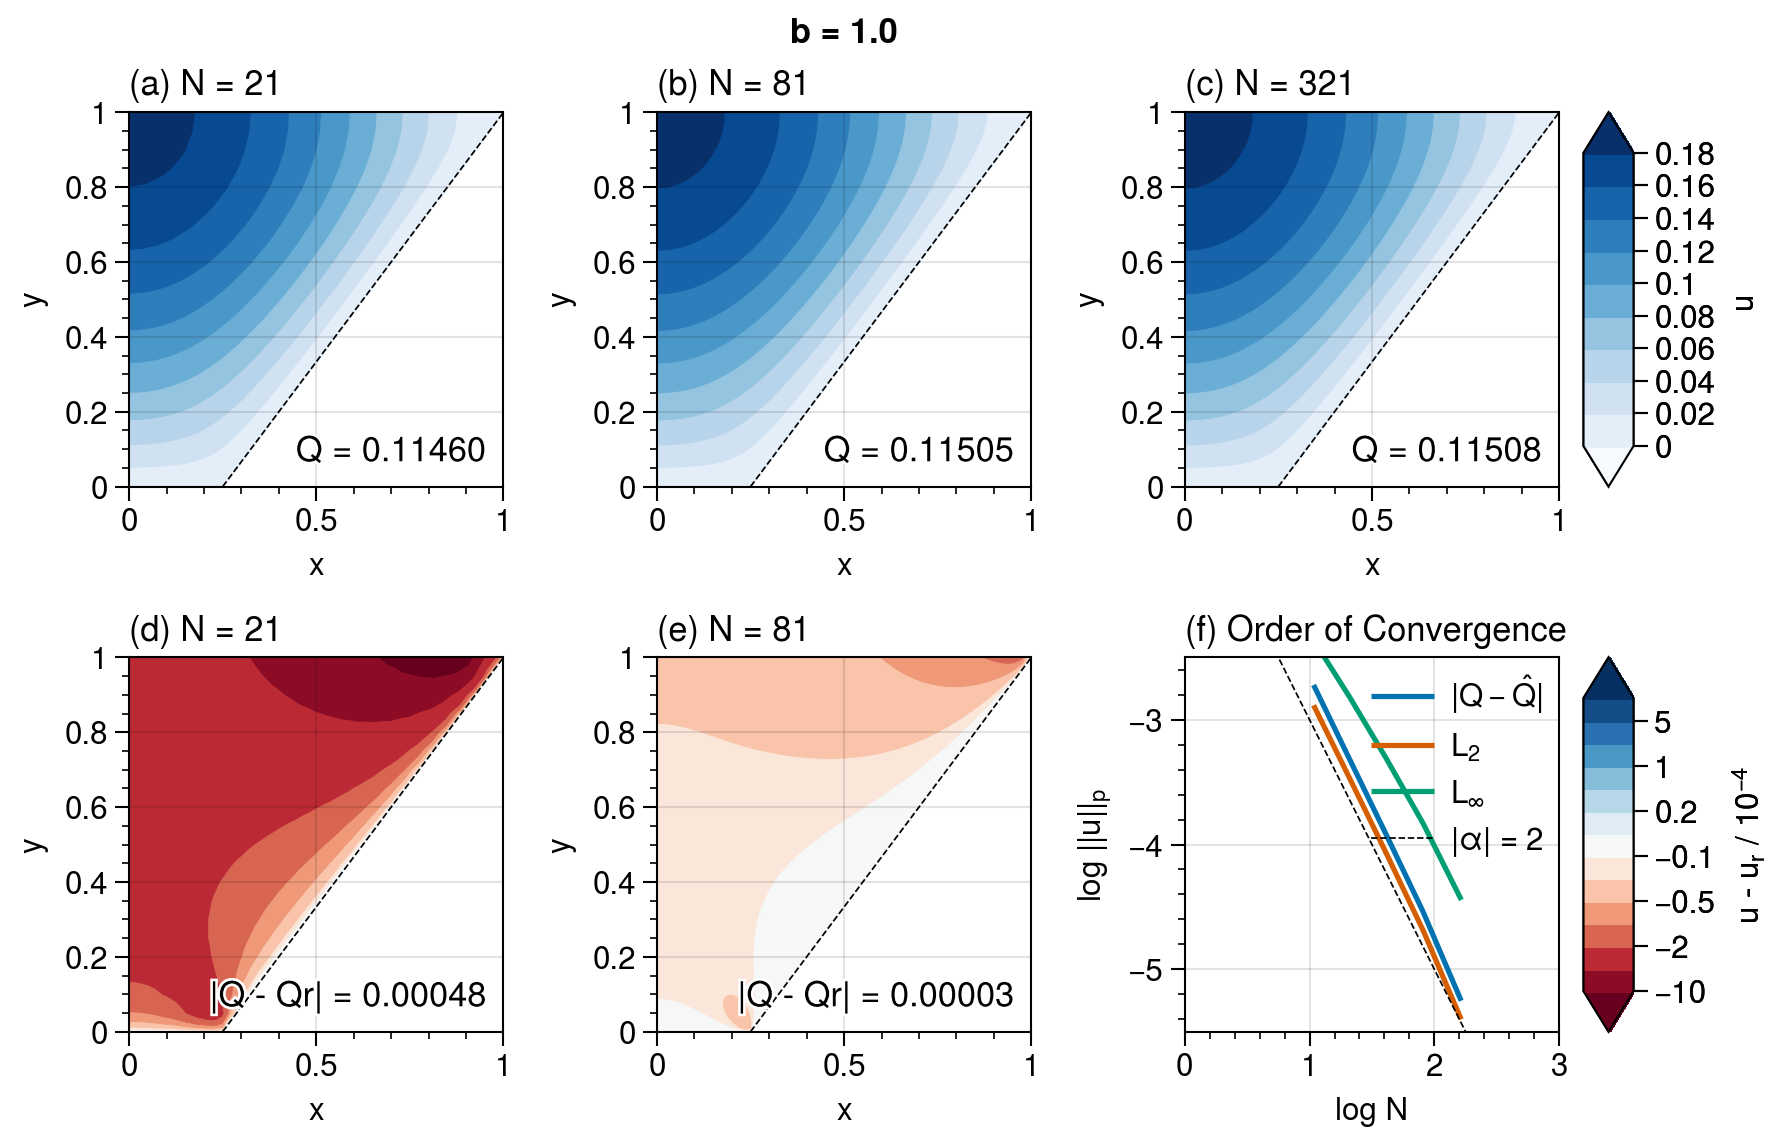
\includegraphics[width=\textwidth]{figures/prj1_qn1f_b0d5.png}\\
    \caption{The numerical solutions for $l=3.0$, $b=0.5$, $h=1.0$, when (a) $N=21$, (b) $N=21$ and (c) $N=321$ (which is taken as the reference).  We see that as $N$ increases the solution at $(x,y) = (0,1)$ increases.  We plot the differences in the numerical solutions of (a) and (b) from (c) in (d) and (e) respectively.  We also (f) plot the rate at which $\norm{u}_p$ converge for $p = 1,2,\infty$, and see that it roughly follows a gradient of -2, and thus the order of convergence is indeed 2.}
    \label{prj1_qn1f_b0d5}
    \end{figure*}
    
    \item This program currently requires as input:
    \begin{itemize}[nolistsep,noitemsep]
        \item The channel geometry parameters $l$, $h$ and $b$
        \item The number of the points $n$ on each side of the domain, we assume that the spacing and domain widths is equal in the $\xi$- and $\eta$ dimensions
    \end{itemize}
    
    How can we extend this program further?  We can do the following
    \begin{itemize}[nolistsep,noitemsep]
        \item Allow specification of the number of points in the $\xi$ and $\eta$ directions separately (i.e. $n\xi$ and $n\eta$ inputs instead of a single parameter $n$)
        \item In the matrix $A$ we construct, we can modify the boundary conditions as required, for example say that there is a lid at the $A'$-$D'$ boundary, we can set $u=0$ instead of $\partial_\eta u = 0$
    \end{itemize}
    
    \item We also calculated the convergence for the problem in part (iv), and plotted it in Fig. \ref{prj1_qn1f_b0d5}f).  We also calculate the convergence for the case where $b=1.0$, and plotted them in a similar manner in Fig. \ref{prj1_qn1f_b1d0}.  We see that for both cases, the gradient of the error in $Q$ and the L-norms have a magnitude of 2, and thus the order of convergence is indeed roughly around 2.

    \begin{figure*}[h!]
    \centering
    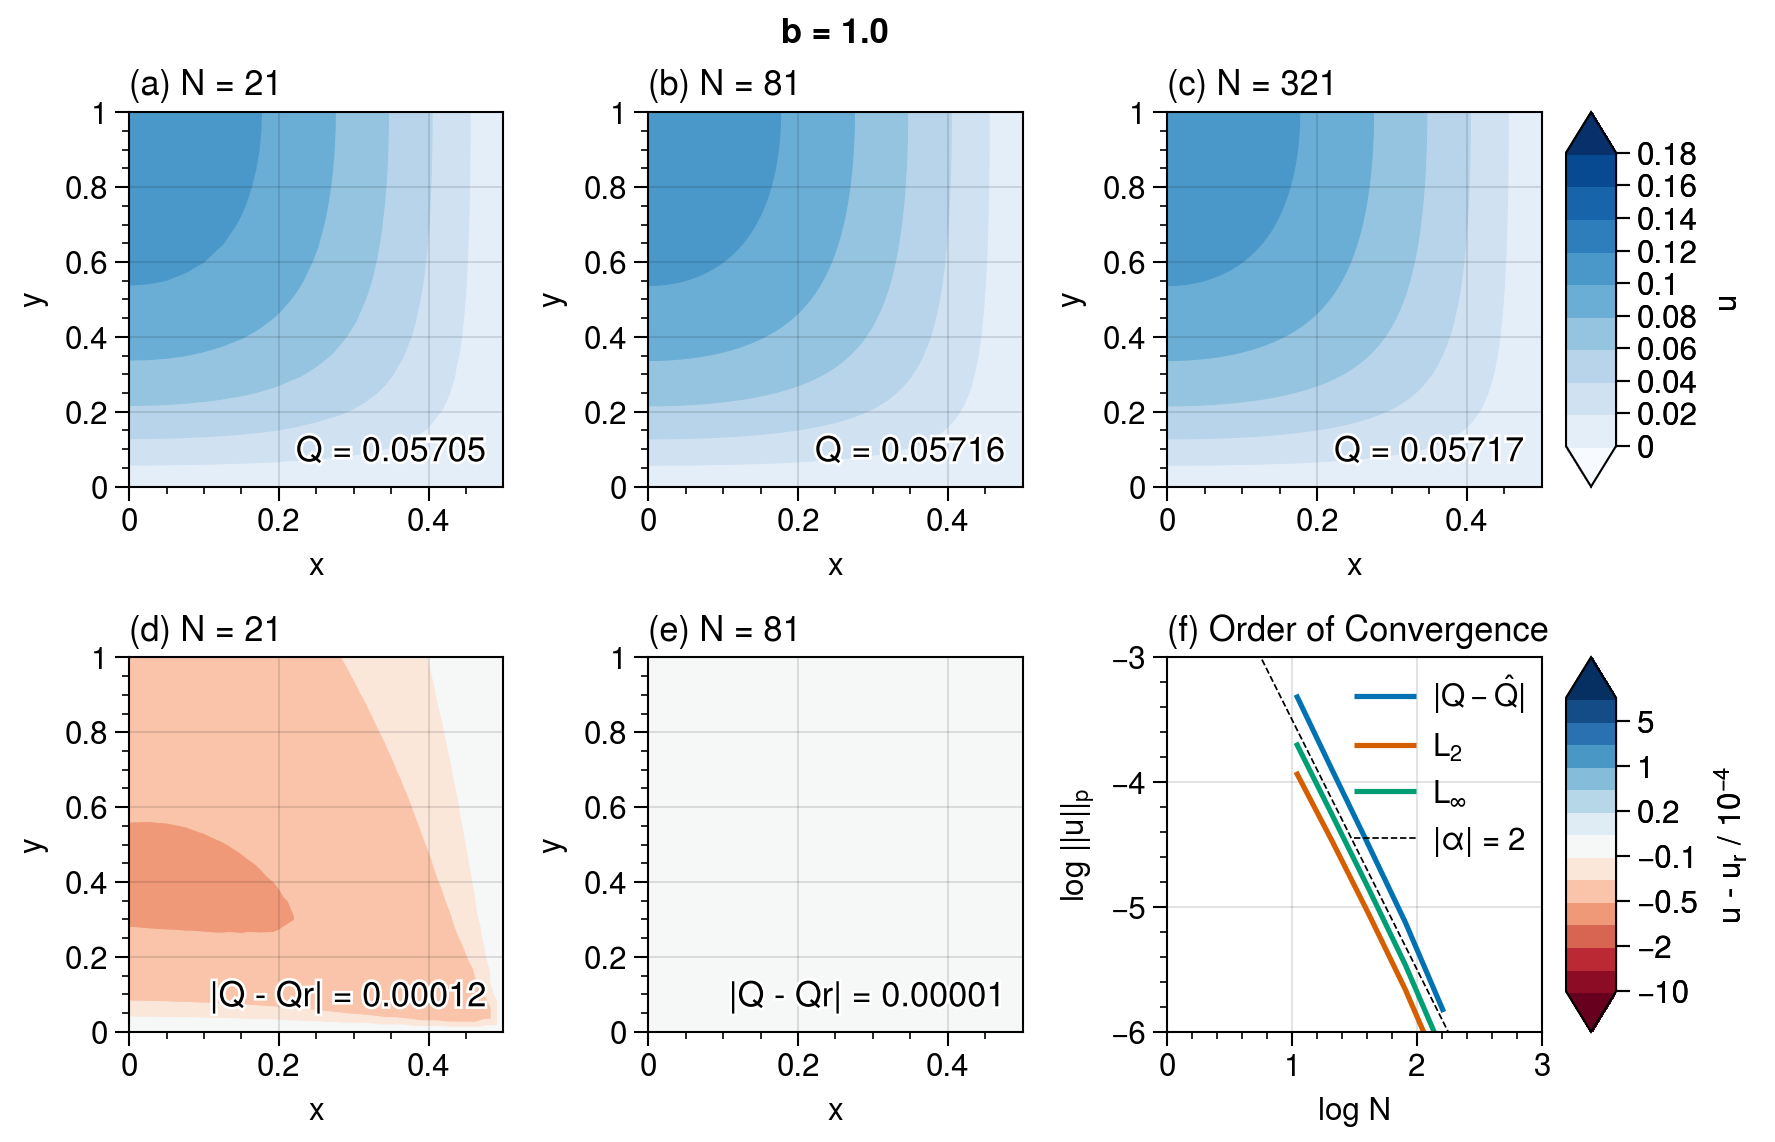
\includegraphics[width=\textwidth]{figures/prj1_qn1f_b1d0.png}\\
    \caption{The numerical solutions for $l=3.0$, $b=1.0$, $h=1.0$, when (a) $N=21$, (b) $N=21$ and (c) $N=321$ (which is taken as the reference).  We see that as $N$ increases the solution at $(x,y) = (0,1)$ increases.  We plot the differences in the numerical solutions of (a) and (b) from (c) in (d) and (e) respectively.  We also (f) plot the rate at which $\norm{u}_p$ converge for $p = 1,2,\infty$, and see that it roughly follows a gradient of -2, and thus the order of convergence is indeed 2.}
    \label{prj1_qn1f_b1d0}
    \end{figure*}
    
    \item We calculate the moment of inertia $I$ and the flow rate $Q$ for a swathe of parameter space over $b$ and $h$ and plot them in Fig. \ref{prj1_qn1g}a,b.  Then, we plot $I$ against $Q$ in Fig. \ref{prj1_qn1g}c to obtain a Pareto curve. We see from the Pareto curve that the flow rate tends to be higher as $I$ increases, but only up to a point.  The maximum $Q$ is given when $b$ is at a maximum, but this peaks when $h \sim 0.9$.  We attribute this to being because the flow rate $Q$ is being restricted by the frictional force caused by the no-slip condition along the boundaries of the channel. 

    \begin{figure*}[h!]
    \centering
    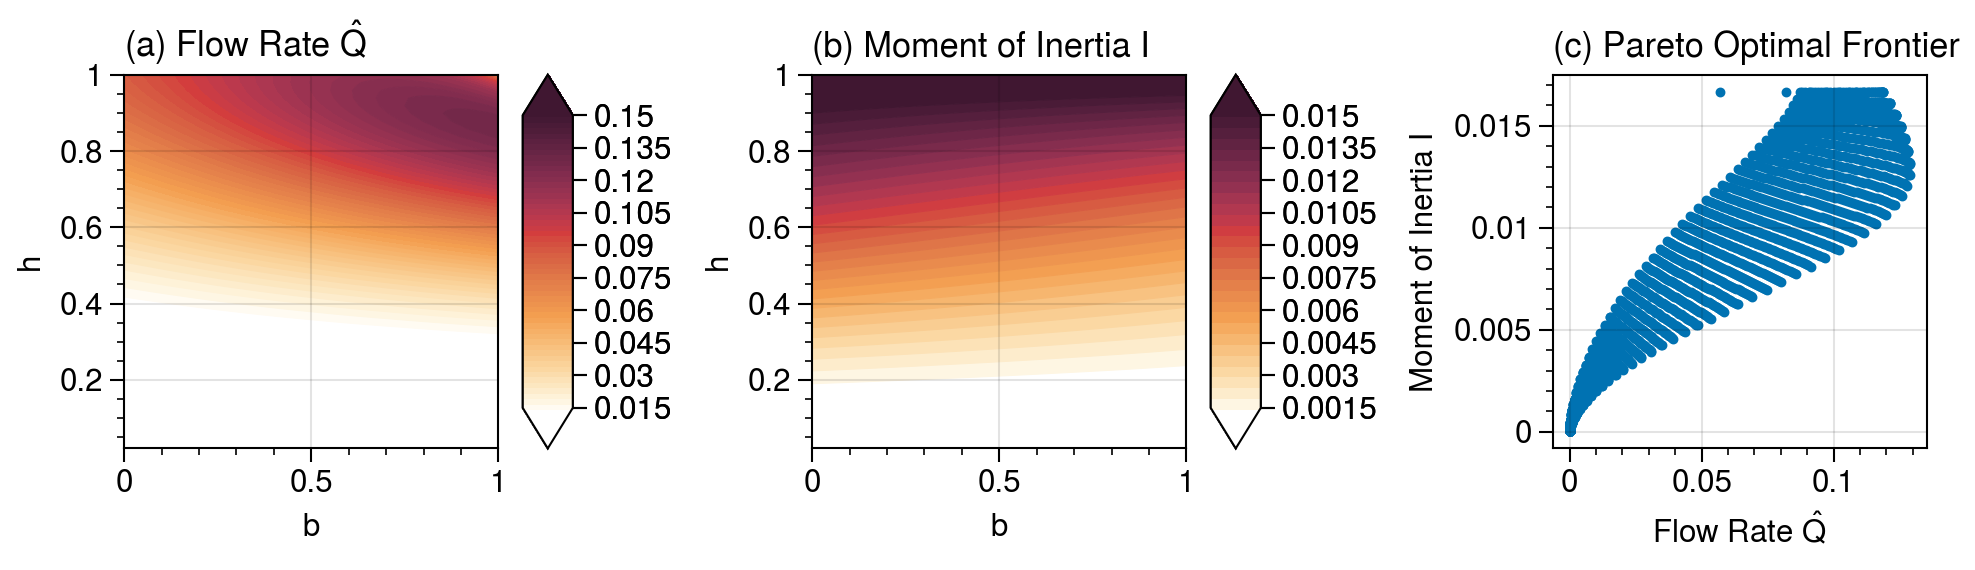
\includegraphics[width=\textwidth]{figures/prj1_qn1g.png}\\
    \caption{We plot (a) the flow rate $Q$, (b) Moment of Inertia $I$ and (c) the Paruto curve by plotting $I$ against $Q$.}
    \label{prj1_qn1g}
    \end{figure*}
    
\end{enumerate}